\documentclass[11pt, a4paper, oneside]{ctexbook}
\usepackage{amsmath, amsthm, amssymb, bm, graphicx, hyperref, mathrsfs, enumitem, geometry, listings, xcolor, listings, fontspec, caption}

% 标题、作者、创建日期
\title{{\Huge{\textbf{PL/SQL学校课程笔记}}}\\ORACLE}
\author{徐鸣飞}
\date{2023年12月27日}

% 设置全局字体
\setmainfont{Times New Roman}

% 设置页面的尺寸和布局。
\geometry{a4paper,scale=0.75}

% 行间距为1.5倍
\linespread{1.5}

% 定义定理环境
\newtheorem{theorem}{定理}[chapter]
\newtheorem{definition}[theorem]{定义}
\newtheorem{lemma}[theorem]{引理}
\newtheorem{corollary}[theorem]{推论}
\newtheorem{example}[theorem]{例}
\newtheorem{proposition}[theorem]{命题}

% 自定义配置
% 设置全局的 enumerate 环境项之间的距离
\setlist[enumerate]{itemsep=5pt, parsep=0pt, leftmargin=20pt, topsep=5pt, partopsep=0pt}

% 定义新环境
% 定义颜色
\definecolor{commentcolor}{RGB}{182,73,1}
% 定义代码
\lstnewenvironment{java}[1][]{
  \lstset{
    language=Java,
    basicstyle=\ttfamily,
    keywordstyle=\color{blue},
    commentstyle=\color{green!60!black},
    stringstyle=\color{commentcolor},
    showstringspaces=false,
    breaklines=true,
    frame=single,
    flexiblecolumns=true,
    backgroundcolor=\color{gray!5},
    numbers=left,
    numberstyle=\tiny,
    #1
  }
}{}
\lstnewenvironment{plsql}[1][]{
  \lstset{
    language=SQL,
    morekeywords={BEGIN,DECLARE,END,IF,ELSE,ELSIF,LOOP,WHILE,PROCEDURE,FUNCTION},
    basicstyle=\ttfamily,
    keywordstyle=\color{blue},
    commentstyle=\color{green!60!black},
    stringstyle=\color{commentcolor},
    showstringspaces=false,
    breaklines=true,
    frame=single,
    flexiblecolumns=true,
    backgroundcolor=\color{gray!5},
    numbers=left,
    numberstyle=\tiny,
    #1
  }
}{}

% 文章开始
\begin{document}

% 生成标题
\maketitle

% 生成目录
\newpage                    %新的一页
\pagenumbering{Roman}       %页码以大写罗马数字形式表示
\setcounter{page}{1}        %设置当前页为第一页
\tableofcontents            %生成目录

% 生成内容
\newpage                    %新的一页
\pagenumbering{arabic}      %页码以阿拉伯数字形式表示
\setcounter{page}{1}        %设置当前页为第一页

% 文章内容
\chapter{导言}
\section{常见数据库}
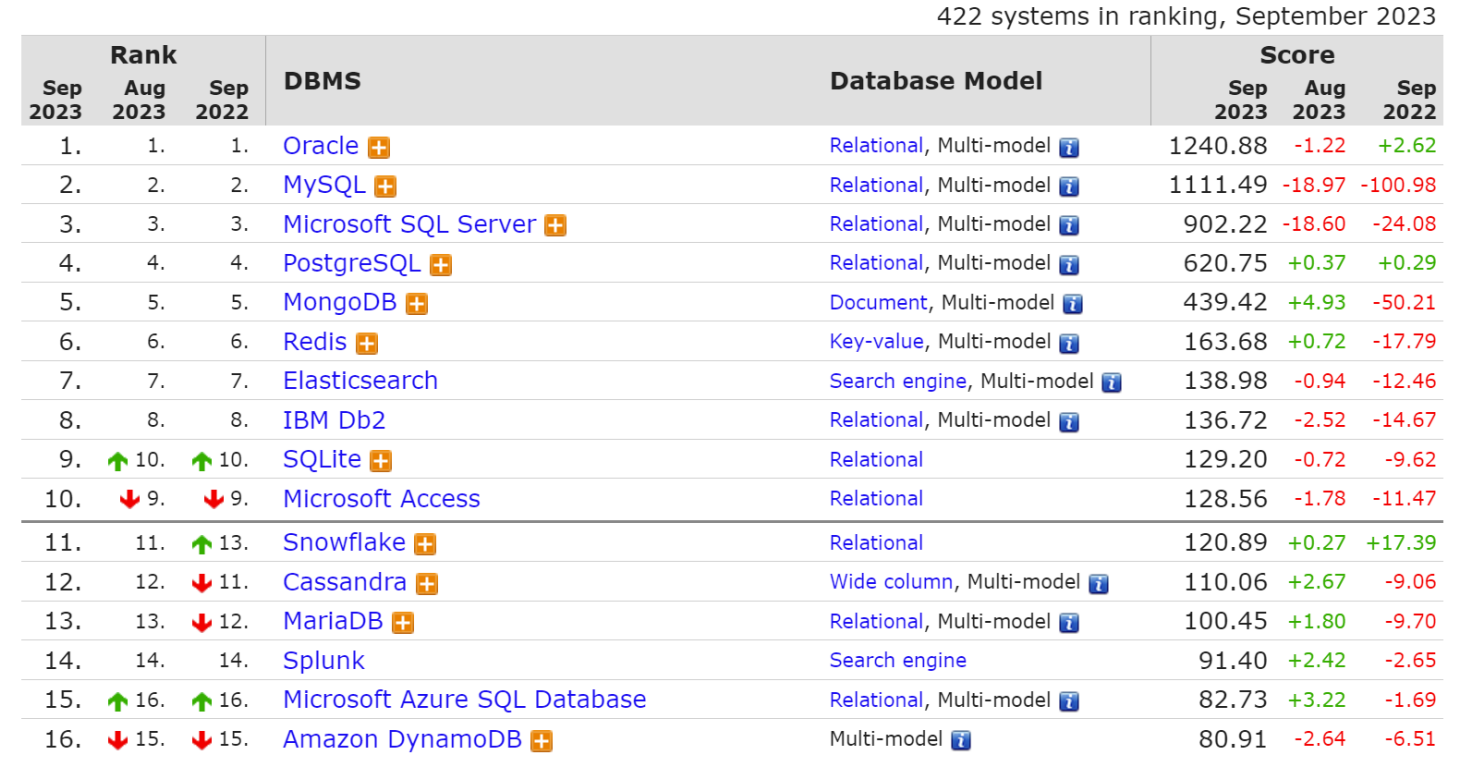
\includegraphics[width=0.9\linewidth]{picture/数据库占比对比.png}
\subsection{关系型数据库}
\subsubsection{MySQL}
MySQL是一款\textbf{开源的关系型数据库管理系统(RDBMS)},由瑞典MySQL AB公司开发,现由Oracle公司维护。以其轻量级、高效、快速的特性而闻名,适用于中小型应用和网站。MySQL支持多平台运行,包括Windows、Linux、macOS等,提供多种存储引擎如InnoDB、MyISAM等,具备良好的扩展性和广泛的社区支持。作为开源软件,MySQL允许用户免费获取、使用和修改其源代码,成为广泛应用于Web开发和其他应用场景的可靠数据库解决方案。
\subsubsection{Oracle}
Oracle是一款\textbf{商业性质的关系型数据库管理系统(RDBMS)},由Oracle公司开发。以其丰富的功能集、高级事务管理、安全性和卓越的性能而著称,适用于大型企业级应用。Oracle数据库支持复杂查询、分布式数据库、以及高并发环境下的大规模数据处理,具备出色的可伸缩性和性能优化特性。作为商业软件,Oracle提供了专业的技术支持、认证体系和咨询服务,成为众多大型组织和企业信赖的数据库解决方案。
\subsection{NoSQL数据库}
\subsubsection{文档型数据库:MongoDB}
\textbf{MongoDB是一种非关系型数据库管理系统(NoSQL DBMS),以其面向文档的存储模型而著称。}由MongoDB公司开发,采用分布式架构和灵活的模式设计,适用于处理大量非结构化或半结构化的数据。MongoDB的数据存储形式为BSON(Binary JSON),支持动态模式,使得数据存储和查询更加灵活。其强大的横向扩展性和自动分片功能使得MongoDB适用于大规模数据存储和处理,尤其在Web应用、大数据和实时分析等场景中表现出色。由于其开源特性,MongoDB拥有庞大的社区支持,为开发人员提供了丰富的资源和工具。
\subsubsection{搜索引擎:Elasticsearch}
\textbf{Elasticsearch是一种分布式数据库管理系统,专注于搜索和分析大规模数据。}作为开源软件,Elasticsearch构建在Apache Lucene之上,采用文档导向的存储模型,以JSON格式存储数据。其核心能力包括实时搜索、结构化查询和复杂分析,使其成为处理实时数据和日志、构建全文搜索引擎以及进行大规模数据分析的理想选择。通过支持分布式架构,Elasticsearch实现了水平扩展,能够应对高负载和大规模数据存储需求。该系统与Kibana等工具的整合形成了ELK堆栈,为用户提供了全面的数据管理、搜索和可视化解决方案。
\subsubsection{key-value数据库:redis}
\textbf{Redis是一款开源、高性能的键值对存储系统,属于NoSQL数据库的一种。}作为内存数据库,Redis将数据存储在内存中,提供了快速的读写访问速度,适用于对性能有严格要求的场景。其特色包括支持多种数据结构(如字符串、哈希表、列表、集合等),原子性操作,发布订阅机制等。虽然主要用于缓存、会话管理和实时数据分析等领域,但由于其快速响应和可持久化存储的能力,也在一些应用中用作主数据库。Redis的灵活性、简单性和高可用性,使其成为各种实时应用和分布式系统的理想选择。
\section{数据库发展趋势}
\subsection{1960s-1980s:层次数据库}
20世纪60年代到80年代的数据库技术被称为“层次结构”,也可以被称为网状结
构,无论标签是什么,这个时代的想法都旨在以树状结构组织数据结构。

\textbf{换而言之,这个时代的数据库技术是将数据存储为相互链接的记录。}
\begin{figure}[htbp]
  \center
  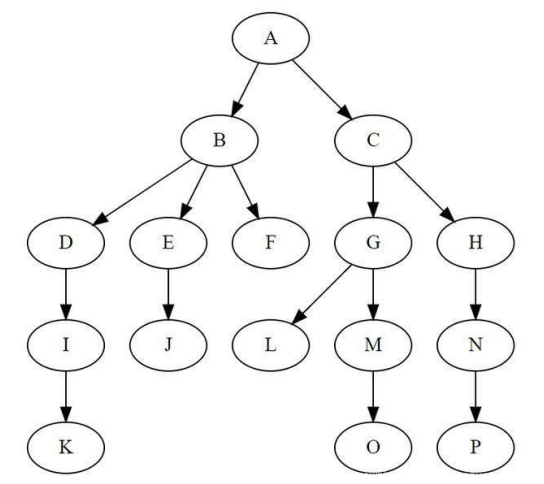
\includegraphics[width=0.5\textwidth]{picture/层次数据库示意图.png}
  \caption{层次数据库示意图}
  \label{fig:hierarchicalDatabase}
\end{figure}
在层次数据库的模型中,数据以节点的形式存在,每个节点可以包含一个或多个字段,形成父子关系。根节点是顶层节点,而叶节点是没有子节点的底层节点。层次数据库适用于需要表示层次结构信息的场景,如组织结构、文件系统等。尽管在过去曾经流行,但由于关系型数据库的普及,层次数据库在现代数据库系统中的应用相对较少。其特点包括数据重复、路径的唯一性以及专门的查询语言用于数据检索和更新。
\subsection{1980s-2000s:实体关系数据库}
实体关系数据库(Entity-Relationship Database)是一种基于实体-关系模型的数据库系统,用于存储和管理数据。在这个模型中,数据以实体(Entity)和实体之间的关系(Relationship)为核心。每个实体都有属性,而实体之间的关系描述了这些实体之间的联系和交互。

实体关系数据库的优势在于其规范化的数据结构、ACID 特性(原子性、一致性、隔离性、持久性)以及使用 SQL(Structured Query Language)进行数据操作和查询的能力。这种数据库模型在处理复杂的关联数据和支持事务处理方面表现出色,因此在各种应用场景中广泛应用,包括企业应用、金融系统、医疗信息管理等。

关系型数据库采用了关系代数的概念,数据以表格(表)的形式组织,每个表表示一个实体,表中的行代表实体的具体实例,而列代表实体的属性。实体之间的关系则通过外键来建立。
\begin{figure}[htbp]
  \center
  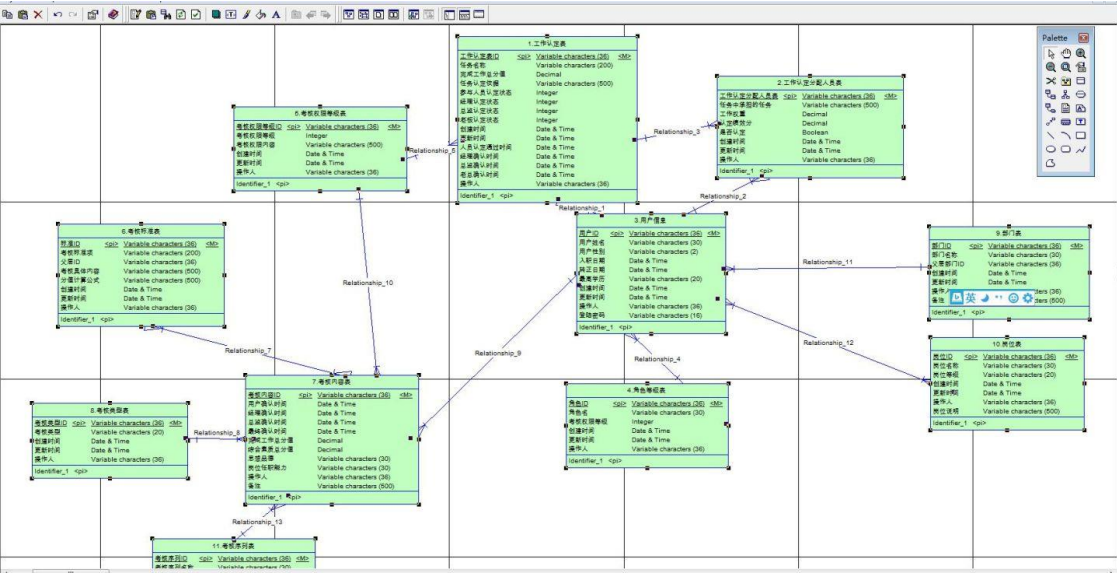
\includegraphics[width=0.5\textwidth]{picture/实体关系数据库示意图.png}
  \caption{实体关系数据库示意图}
  \label{fig:relationDatabase}
\end{figure}
\subsection{2000s-2020s:NoSQL}
NoSQL为Not Only SQL的缩写,是对不同于传统的关系型数据库的数据库管理系统的统称。

\textbf{网络上的数据本质上不是表格的结构。}

NoSQL常用于超大规模数据的存储(例如谷歌或Facebook每天为他们的用户收集万亿比特的数据)。这些类型的数据存储不需要固定的模式,无需多余操作就可以横向扩展。

\begin{center}
  \begin{minipage}{0.99\textwidth}
    \center
    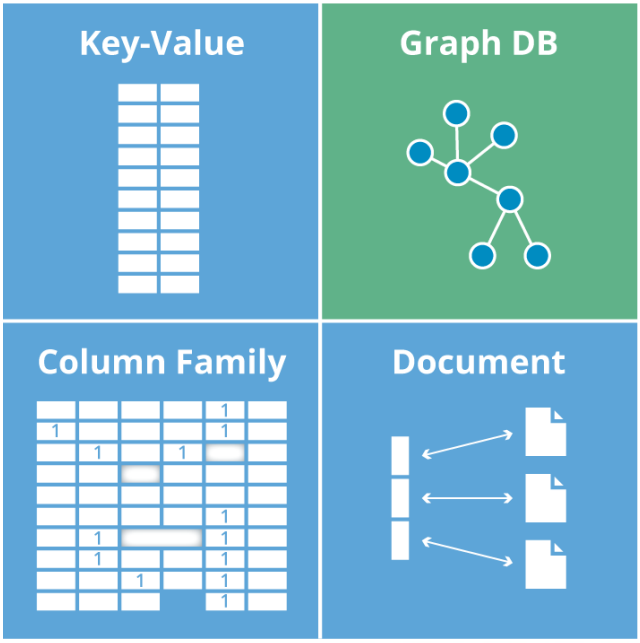
\includegraphics[width=0.5\textwidth]{picture/NoSQL数据库示意图.png}
    \captionsetup{hypcap=false}
    \captionof{figure}{NoSQL数据库示意图}
    \label{fig:NosqlDatabase}
  \end{minipage}
\end{center}

\subsection{2020s-未知:图数据库}
这个创新时代正在从存储系统的效率转向\textbf{从存储系统包含的数据中提取价值}。

\textit{即价值从效率转移到高度连接的数据资产中衍生。}

\section{Oracle架构}

\section{PL/SQL介绍}
\subsection{概述}
\textbf{PL/SQL(Procedural Language/Structured Query Language)}:一种\textbf{过程化编程语言},专门用于\textbf{Oracle数据库系统}。它将SQL(Structured Query Language)语句与结构化程序设计语言(如条件、循环等)相结合,提供了一种强大的方式来处理和操作数据库中的数据。


% 文章结束
\end{document}